%%%%%%%%%%%%%%%%%%%%%%%%%%%%%%%%%%%%%%%%%%%%%%%%%%%%%%%%%%%%%%%%%%%%%%%%%%%%%%%%
%% INTRODUCTION
%%%%%%%%%%%%%%%%%%%%%%%%%%%%%%%%%%%%%%%%%%%%%%%%%%%%%%%%%%%%%%%%%%%%%%%%%%%%%%%%


This chapter presents the method to evaluate the reliability property of
product lines following a feature-family-based
strategy~\cite{thum_classification_2014}.  It consists of three key steps, as
shown in Figure~\ref{fig:evaluationApproach}. 


First, the \emph{transformation} step maps UML behavioral diagrams with variability
into a graph structure called Runtime Dependency Graph (RDG), whose nodes
represent the behavioral fragments and store corresponding FDTMCs (i.e. the
probabilistic behavioral model), meanwhile the edges represent the runtime
dependencies between such models.  Next, the \emph{feature-based} evaluation step
leverages parametric model checking to analyze each FDTMC in isolation against a
reliability property, by abstracting the existing runtime dependencies between
them.  This results in rational expressions~\cite{HahnHZ10} (hereafter referred
to simply as \textit{expressions}), each giving the reliability of an FDTMC as a
function of the reliabilities of the FDTMCs on which it depends.  Lastly, the
\emph{family-based} evaluation step follows a topological sorting of the runtime
dependency graph, computing the reliability value of each configuration by
evaluating the expression in each node and reusing the evaluation results
previously computed for the nodes on which it depends.  This step also considers
the variability model of the product line in question to prune invalid
configurations. The following subsections describe these steps in detail, guided
by the example of Section~\ref{sec:runningExample}.


\begin{figure}[hbt]
	\centering
	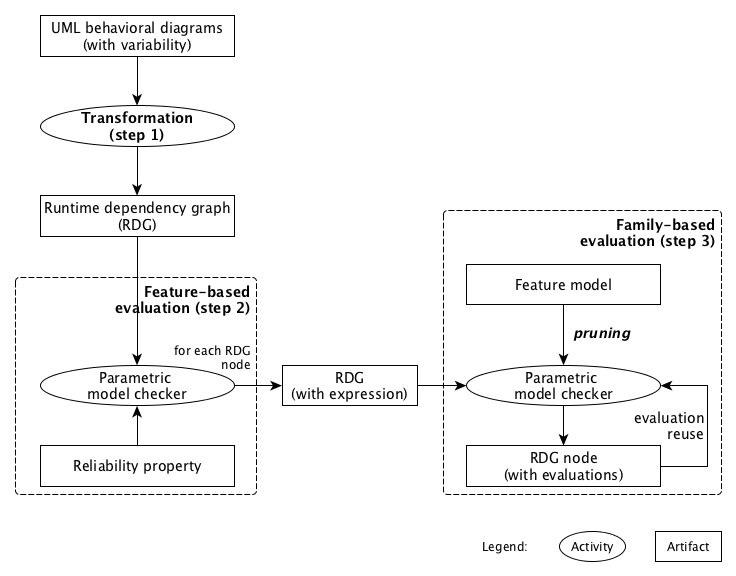
\includegraphics[width=\columnwidth]{img/evaluationApproach}
	\caption{Feature-family-based approach for efficient reliability
	  analysis of product lines.} 
	\label{fig:evaluationApproach}
\end{figure}


%%%%%%%%%%%%%%%%%%%%%%%%%%%%%%%%%%%%%%%%%%%%%%%%%%%%%%%%%%%%%%%%%%%%%%%%%%%%%%%%
%% TRANSFORMATION
%%%%%%%%%%%%%%%%%%%%%%%%%%%%%%%%%%%%%%%%%%%%%%%%%%%%%%%%%%%%%%%%%%%%%%%%%%%%%%%%
\section{Transformation   \label{subsec:transformation}}


To perform the reliability analysis of a given product line, the proposed method
first composes its inherent variability and probabilistic behavior into a data
structure named Runtime Dependency Graph (RDG), which is then used for analysis
in further steps.  The probabilistic behavior can be derived from UML behavioral
models, representing the runtime interactions between software components,
enriched with reliability information for such interactions.  Details on the
behavioral models, the RDG, and the transformation of the former into the latter
are provided next.


% To perform the reliability analysis of a software product line, it is first
% necessary to consider its inherent variability jointly with its probabilistic
% behavior.  Such behavior can be derived from models representing the runtime
% interactions among software components, enriched with probabilistic
% information for such interactions.  Since UML is well-known for representing
% different facets of a software, its behavioral models can be used by the
% transformation step to create probabilistic models which consider the
% variability of the software product line. The interdependencies represented at
% the behavioral models are also considered by transformation step and,
% considering a behavioral model can be reused by several other behavioral
% models, such interdependencies are captured by a graph-similar data structure.

% Figure \ref{fig:oxygenationSituation} depicts the optional behavior for
% processing information regarding Oxygenation at the BSN example. Such behavior
% is represented by a sequence diagram whose messages are annotated with
% probabilistic values, and it depends on two other behavioral models.




%%%%%%%%%%%%%%%%%%%%%%%%%%%%%%%%%%%%%%%%
\subsection{Behavioral Models \label{subsec:behavioralModels}}

The evaluation approach considers the coarse-grained behavior of a product line
is represented by a UML activity diagram, with each activity being refined into
a sequence diagram~\cite{rodrigues_modeling_2015}. The activity diagram is
useful for representing whether the activities are performed in a sequential or
parallel manner, whereas sequence diagrams represent how the probabilistic
behavior of the interactions between software components varies according to the
configuration space of the product line. To represent probabilistic behavior,
each message in a sequence diagram is annotated with a probability value that
represents the reliability of the communication channel---i.e., the probability that the
interaction succeeds---by using the UML MARTE profile~\cite{uml-marte-profile}
(e.g., \textit{prob} tags in Figure \ref{fig:oxygenationSituation}).


Without loss of generality, behavior variability is defined by
\textit{behavioral fragments}, each of which can be an activity diagram (that
has an associated sequence diagram),  a sequence diagram, or an optional
combined fragment within a sequence diagram such that this fragment has a  guard
condition denoting its presence condition~\cite{czarnecki_verifying_2006}.  These
conditions are propositional logical statements defined over features, that
denote the set of configurations for which the guarded behavior is present.
Optional combined behavioral fragments can be nested, which allows representing
behavioral variability at several levels.  

% Figure~\ref{fig:behavioralFragmentComposition} shows the relations between
% such elements for representing the whole system behaviors: a
% \textit{behavioral fragment} can be specialized into an activity diagram that
% has an associated sequence diagram, but also into a \textit{sequence diagram}
% or an \textit{optional combined fragment}, each of which can enclose other
% optional combined fragments.

Note that the behavioral variability expressed by optional fragments may be
implemented in two distinct ways: 1)  in case the fragment's guard condition is
expressed by an atomic proposition (i.e., a single feature), the feature may be
implemented in its own module, which characterizes a compositional  product
line; 2) if the guard condition is a propositional formula comprising two or
more features, such tangled behavior can be implemented in an annotation-based
style by using, for example, the \texttt{\#ifdef} and \texttt{\#endif} macros of
the C preprocessor. Therefore, the hereby presented method can be applied to
analyze both compositional and annotation-based software product lines.

% \begin{figure}[hbtp] \centering
%   %\includegraphics[width=0.7\columnwidth]{images/behavioralFragmentComposition}
%   \centering
%   \footnotesize
\centering
\begin{tikzpicture}[baseline, level 1/.style={sibling distance=30mm}]
\node[rectangle, draw=black](BF){Behavioral Fragment}
  child[open triangle 45-, thick]{node[rectangle, draw=black](AD){Activity\\ Diagram}}
  child[open triangle 45-,, thick]{node[rectangle, draw=black](SD){Sequence\\ Diagram}}
  child[open triangle 45-,, thick]{node[rectangle, draw=black](OCF){Optional \\combined fragment}};
  
  \draw [-latex, thick](AD) -- node[below, near end, draw=none]{1} (SD);
  \draw [-diamond](OCF.north) |- +(2.3cm,0.5cm) |- (OCF.east);
  \draw [diamond-](SD) -- (OCF);
\end{tikzpicture}

%   \caption{Associations between 
%     \textit{Behavioral Fragment}, \textit{Sequence Diagram}, and \textit{Optional
%     Combined Fragment} for representing nested behavioral structures.}
%   \label{fig:behavioralFragmentComposition} 
% \end{figure}

%In particular, a behavioral fragment is considered an unit of modeling to which
%it is possible to assign a presence condition~\cite{czarnecki_verifying_2006}
%representing the software product line's variability. %It is related to the
%following UML elements: activity diagrams, sequence diagrams and the optional
%combined fragment of sequence diagrams. %, parallel and loop combined fragments
%of sequence diagrams.  Each one of such behavioral elements is considered as an
%isolated behavioral fragment analyzed only for configurations fulfilling a
%propositional formula representing its presence condition.  

% Presence condition plays a major role in our approach because it increases the
% expressiveness level of variability at the behavioral models of a software
% product line. Indeed, as presence conditions are related to behavioral
% fragments' guards, it is possible to define the set of configurations to be
% considered for each behavioral fragment representing the behavior of a
% software product line.  In particular, presence conditions enable modeling
% feature interaction~\cite{apel_feature-oriented_2013}, by representing the
% specific behavior for a product which has two or more interacting features. 

As an example, Figure~\ref{fig:bsnControlLoop} shows a UML activity diagram
describing, at a high level, the behavior of all products of the BSN product
line.  The behavior corresponding to the activity \textit{system identifies
situation} is modeled by an associated sequence diagram, \emph{partially}
depicted in figures~\ref{fig:oxygenationSituation} and \ref{fig:temperatureSituation}.

The sequence diagram shown in Figure \ref{fig:oxygenationSituation} presents
three behavioral fragments whose presence conditions are  the atoms
\texttt{oxygenation}, \texttt{memory}, and \texttt{sqlite}. The outermost
behavioral fragment represents the optional behavior for processing the
oxygenation information in the BSN product line, and it varies according to two
nested behavioral fragments. These latter are optional combined fragments
related to \textit{Sqlite} and \textit{Memory} features of the feature model in
Figure~\ref{fig:fm} and, jointly with this model's constraints, ultimately
represent alternative behavior for data persistence. Analogously, the sequence
diagram shown in Figure~\ref{fig:temperatureSituation} has its behavior varying
in terms of \emph{Temperature}, \emph{SQLite} and \emph{Memory} features due the optional
combined fragments also has the guards defined by the atoms
\texttt{temperature}, \texttt{sqlite} and \texttt{memory}, respectively. 

% The sequence diagram shown in Figure \ref{fig:oxygenationSituation} presents
% three behavioral fragments whose presence conditions are  the atoms
% $oxygenation$, $memory$, and $sqlite$. The outermost fragment represents the
% optional behavior for processing the oxygenation information in the BSN, and
% it varies according to two nested behavioral fragments. These fragments
% represent optional behaviors for data persistence and are related to Sqlite
% and Memory features of the Feature Model. 






%%%%%%%%%%%%%%%%%%%%%%%%%%%%%%%%%%%%%%%%%%%%%%%%%%%%%%%%%%%%%%%%%%%%%%%%%%%%%%%%
%% RUNTIME DEPENDENCY GRAPH
%%%%%%%%%%%%%%%%%%%%%%%%%%%%%%%%%%%%%%%%%%%%%%%%%%%%%%%%%%%%%%%%%%%%%%%%%%%%%%%%
\section{Runtime dependency graph (RDG) \label{sec:runtimeDependencyGraph}}

A Runtime Dependency Graph (RDG) is a behavioral representation for variable
systems, which combines the configurability view of a product line (expressed by
presence conditions) with its probabilistic behavior (expressed by FDTMCs).
Formally, it can be defined as follows.

\begin{definition}[RDG] A Runtime Dependency Graph $\mathcal{R}$ is a directed
	acyclic graph $\mathcal{R} = (\mathcal{N}, \mathcal{E}, x_0)$, where
	$\mathcal{N}$ is a set of nodes, $\mathcal{E} : \mathcal{N} \cdot
	\mathcal{N}$ is a set of directed edges that denote a dependency
	relation, and $x_0 \in \mathcal{N}$ is the \emph{root} node with
	in-degree 0.  An RDG node $x \in \mathcal{N}$ is a pair $x = (m, p)$,
	where $m$ is an FDTMC representing a probabilistic behavior and $p$ is a
	propositional logic formula that represents the presence condition
	associated with $m$.  
\end{definition}

To build an RDG for a software product line, the method extracts the
configurability and probabilistic information only from the UML behavioral
diagrams, such that each RDG node is associated with an FDTMC derived from a
behavioral fragment (c.f. Figure~\ref{fig:nestedBehavioral}) and its presence
condition.  Since it is considered that the
UML activity diagram represents the product line's \textit{coarse-grained
behavior} executed by all products and each activity is further refined
(detailed) into its respective sequence diagram, two aspects of the method
deccurs.  First, the behavioral variability is not considered at the
representation at system level, which implies its related RDG nodes have
\textit{true} as presence condition (i.e., it is satisfied for all products).
Finally, as an activity has as an association with its refining sequence
diagram, such association is represented in the RDG by an edge. Therefore, edges
represent dependencies between nodes, which are due to refinement or nesting
relations between the respective behavioral fragments.  The RDG nodes that do
not depend on any other node are called \textit{basic}.  The ones with
dependencies are called \textit{variant} nodes, which are represented with
outgoing edges directed to the RDG nodes on which they depend. 

The structure of UML sequence diagrams is tree-like, which suggests a tree could
be a better model of their dependencies.  Nonetheless, applications sometimes
have behavioral fragments replicated throughout UML models. For instance, the
data persistence behavior in Figure \ref{fig:oxygenationSituation} is present in
all fragments that denote sensor information processing including the temperature information processing represented by Figure~\ref{fig:temperatureSituation}. In this approach,
redundant fragments are represented by a single RDG node, with as many incoming
edges as its number of replications.  When performing this reuse, the resulting
graph will be acyclic, because the original UML model is a finite hierarchy.

Figure~\ref{fig:rdgOxygenation} illustrates an excerpt of the BSN product line's
RDG that represents the behavioral fragments of
figures~\ref{fig:oxygenationSituation} and \ref{fig:temperatureSituation}. As
the fragments related to \textit{Sqlite} and \textit{Memory} features are nested
inside the fragments related to the \textit{Oxygenation} and \emph{Temperature}
features, the RDG for these fragments represents the dependencies between their
respective nodes. The behavioral fragments related to \textit{Oxygenation} and
\emph{Temperature} are part of the sequence diagram representing the behavior of
the activity \textit{system identifies situation}.  Therefore, these relations
are also represented by the edges from the node \texttt{rSituation}  to the
nodes \texttt{rOxygenation} and \texttt{rTemperature}, respectively. For
brevity, it is not represented the internal structure of the nodes and the
remaining RDG nodes (indicated by suspension points in Figure~\ref{fig:rdgOxygenation}).




\subsubsection{From Behavioral Models to RDG}
\label{subsubsec:umlToRDG}

The transformation from behavioral models to an RDG can be described at two
abstraction levels: the RDG topology and the generation of probabilistic models.
Listings \ref{lst:transformAD} and \ref{lst:transformSD} both depict the
transformation process from the topological point of view.  Note that this step
relies on uniquely generated identifiers for the behavioral models(line
\ref{line:rootRdgNodeCreation}), which are
then used as identifiers for the respective RDG nodes.

The process starts by calling the \texttt{transformAD} method
(Listing~\ref{lst:transformAD}), passing as argument the single activity diagram
that embodies the coarse-grained behavior of the product line.  This method
creates the \emph{root} node (Line~\ref{line:rootRdgNodeCreation}), setting its
presence condition to \texttt{true} (i.e., the overall behavior must always be
present; Line~\ref{line:truePresenceCondition}).  The root's probabilistic model
is then generated by processing the input diagram with the
\texttt{ad\-To\-FDTMC} method (Line~\ref{line:adToFDTMC}), which will be
presented later.  Then the approach creates an RDG node for each sequence
diagram that refines an activity (denoted by the property
\texttt{act.se\-quence\-Di\-a\-gram}), subsequently creating edges that mark
them as dependencies of the \emph{root} node
(Line~\ref{line:transformActivity}).  Note that the \textit{root} node is the
only RDG node created by the \texttt{transformAD} method, so the root's FDTMC
models the behavior represented by the activity diagram.

\begin{lstlisting}[label={lst:transformAD},
                   caption={Activity diagram transformation},
                   float,
                   breaklines,
		   belowcaptionskip=0.2cm]
RDGNode transformAD(ActivityDiagram ad) {
    RDGNode root = new RDGNode(ad.id);(*@\label{line:rootRdgNodeCreation}@*)
    root.model = adToFDTMC(ad);(*@\label{line:adToFDTMC}@*)
    root.presenceCondition = true;(*@\label{line:truePresenceCondition}@*)
    for (Activity act : ad.activities) {
        root.addDependency(transformSD(act.sequenceDiagram));(*@\label{line:transformActivity}@*)
    }
    return root;
}
\end{lstlisting}

The creation of RDG nodes for sequence diagrams is similar: the method
\texttt{trans\-form\-SD} (Listing~\ref{lst:transformSD}) takes a behavioral
fragment as input and then creates a new RDG node whose FDTMC is derived by the
\texttt{sd\-To\-FDTMC} method (Line~\ref{line:sdToFDTMC}). In this case, since
behavioral fragments encode variability, their guard is assigned as the presence
condition of the newly created node (Line~\ref{line:guardCondition}). As with
refined activities, the approach creates RDG nodes for nested behavioral
fragments and set them as dependencies of the node at hand (Line
\ref{line:transformFragment}).

The reuse of behavior briefly and previously mentioned in
this section is performed by calling the static method
\texttt{RDG\-Node.\-reuse} (Listing \ref{lst:transformSD},
Line~\ref{line:nodeReuse}). This function maintains a registry of all RDG nodes
created, and then searches among them for one that is considered
\emph{equivalent} to the one just created. This notion of equivalence is
comprised of three conditions: (a) equality of presence conditions; (b) equality
of FDTMCs; and (c) recursively computed equivalence of dependencies.

The sequence diagrams of figures~\ref{fig:oxygenationSituation} and
\ref{fig:temperatureSituation} illustrate such result opportunity. The optional
fragments related to the \emph{SQLite} feature on both sequence diagrams fulfill
the three conditions aforementioned for behavioral reuse: both fragments have
the same guard condition (\texttt{SQLite}), are comprised of the same messages
sequence ([\texttt{persist},\texttt{replyPersist}]) and have the same set of
dependencies (in this specific case, the $\emptyset$ set as they are basic
nodes). The same rationale holds
for the fragment related to the \emph{Memory} feature. Such behavioral reuse
allows reusing both models and evaluations for such fragments, fact that is
represented by the incoming edges to its respective nodes in
Figure~\ref{fig:rdgOxygenation}.

\begin{lstlisting}[label={lst:transformSD},
                   caption={Sequence Diagram transformation},
                   float,
                   breaklines,
		   belowcaptionskip=0.2cm]
RDGNode transformSD(BehavioralFragment sd) {
    RDGNode thisNode = new RDGNode(sd.id);
    thisNode.presenceCondition = sd.guard;(*@\label{line:guardCondition}@*)
    thisNode.model = sdToFDTMC(sd);(*@\label{line:sdToFDTMC}@*)
    for (BehavioralFragment frag : sd.optFragments) {
        thisNode.addDependency(transformSD(frag));(*@\label{line:transformFragment}@*)
    }
    return RDGNode.reuse(thisNode);(*@\label{line:nodeReuse}@*)
}
\end{lstlisting}



%Thus the transformation step is the responsible for creating the RDG from the
%UML behavioral models of a software product line, representing accordingly the
%dependencies, the probabilistic behavior and the presence conditions
%represented on such models. Despite the transformation being carried out at
%once from the behavioral models, it can be seen as being conducted in two
%distinct steps. The first step's role is responsible for creating the topology
%of the RDG by extracting the refinement and nesting relations from the UML
%behavioral models. The second step role's is the responsible for filling each
%RDG node with the probabilistic model and the presence condition of its related
%behavioral fragment. 

%Considering the behavior of a software product line is coarse-grained
%represented by a single activity diagram whose activities are later refined by
%sequence diagrams, the first step's role is to create a root RDG node
%representing how the activities are performed by the software product line, one
%RDG node for each activity represented at activity diagram and fill each node
%with its probabilistic model. Such transformation is described by the Listing
%\ref{lst:transformAD}. The function \texttt{transformAD} creates an RDG node
%for the incoming activity diagram (line 2) and then assigns its presence
%condition and probabilistic model (lines 3-4). As the root node represents how
%activities are executed by the software product line and it is not restricted
%to any configurations subset, its probabilistic model is given by the
%transformation of the activity diagram into an FDTMC (line 3) and its presence
%condition is equal to \texttt{true} (line 4). Then, for each activity
%represented at the activity diagram an RDG node is created whose probabilistic
%model is given by transforming its related sequence diagram into an FDTMC (line
%6). As root node depends on such nodes, an edge is created between them for
%representing the dependencies (line 7). Therefore the listing
%\ref{lst:transformAD} is the responsible for creating the RDG nodes
%representing the refinement of each activity and the edges representing how
%such nodes affect the probabilistic model of the root node. 

%Sequence diagram is used for representing the probabilistic behavior due
%interactions among the software components of a software product line. For such
%diagram it is important consider how its behavior is defined and, in case
%behavioral fragments are used for representing behavior variability, it is also
%important consider how such fragments are related among them. Listing
%\ref{lst:transformSD} presents an algorithm for performing the transformation
%of Sequence Diagrams into an RDG. The role for function \texttt{transformSD} is
%to create an RDG node for each sequence diagram it receives for analysis (line
%2). As the guard condition of the sequence diagram is a propositional formula
%defined in terms of features, it is assigned to the RDG node's presence
%condition (line 3). After, the interactions between software components
%described in the sequence diagram, except the behavior defined by its
%behavioral fragments, are transformed into a probabilistic model (line 4). As a
%sequence diagram may contains behavioral fragments in its structure, such
%relation characterizes as a behavioral fragment nesting. Therefore for each
%behavioral fragment represented in a sequence diagram an RDG node and an edge
%must be created for representing the dependency between the probabilistic
%behavior of such nodes (lines 5-7). As each behavioral fragment is a sequence
%diagram, which may or not contains other behavioral fragments, it must also be
%transformed by applying the recursive function \texttt{transformSD}.


%\begin{figure}[t]
%  \centering
%  \begin{subfigure}[t]{0.20\textwidth}
%    \resizebox{\linewidth}{!}{
%    \begin{tikzpicture}
%	    \centering
%	    %\begin{tikzpicture}
% \draw[help lines] (0,0) grid +(3, 1);
% \draw[help lines] (0,0) grid +(3,-1);
\node[adStart](start){};
\node[initial, thick](initial) at (3,0){(\textit{init})};
\node[thick](regular) at (5,0){};
\node[error,thick](error) at (5,-2){(\textit{error})};
\draw[thick, dashed](1,1) -- (1,-2);
\draw[thick, ->, line width=1pt] (1.5,0) -- (initial.west);
\draw[thick, ->, line width=1pt] (initial.east) -- node[draw=none, rectangle, above]{$1.0$}(regular.west);
\draw[thick, ->, line width=1pt] (initial.south) |- node[draw=none, rectangle, auto]{$0.0$}(error.west);
%\end{tikzpicture}

%    \end{tikzpicture}}
%    \caption{Initial node.}
%    \label{fig:AD_initial_node}
%  \end{subfigure}
%  ~
%  \begin{subfigure}[t]{0.45\textwidth}
%    \resizebox{\linewidth}{!}{\begin{tikzpicture} \centering
%	    %\begin{tikzpicture}[scale=0.6]
%%%%%%%%%%%%%%%%%%% HELP LINES
% \draw[help lines] (0,0) grid +(6,1);
% \draw[help lines] (0,0) grid +(6,-1);
%%%%%%%%%%%%%%%%%%% NODES
\node[fill=none, draw=none](transp1) at (-1.5,0){$\dots$};
\node[adActiv](activity) at (0.5,0) {Activity};
\node[fill=none, draw=none](transp2) at (2.5,0){$\dots$};

\node[circle, dashed](current) at (4, 1) {};
\node[circle](next) at (6, 1) {};
\node[error, circle, dashed](error) at (6,-1) {(\textit{error})};

\node[rectangle, draw=none, fill=gray!50](constraint) at (5,-2.5){$rActivity \in [0,1]$};

\draw[thick, dashed](3,1) -- (3,-1);
\draw[thick,->, line width=1pt](transp1.east) -- (activity.west);
\draw[thick,->, line width=1pt](activity.east) -- (transp2.west);
\draw[thick,->, line width=1pt](current.east) -- node[midway, yshift=0.3cm, fill=none, draw=none]{rActivity} (next.west);
\draw[thick,->, line width=1pt](current.south) |- node[midway, yshift=-0.3cm, fill=none, draw=none]{1-rActivity}(error.west);

%\end{tikzpicture}
 \end{tikzpicture}}
%    \caption{Activity.}
%    \label{fig:AD_activity}
%  \end{subfigure}
%
%  \vspace{0.5cm}
%  \begin{subfigure}[t]{0.45\textwidth}
%    \centering
%    \resizebox{\linewidth}{!}{\begin{tikzpicture}
%    %%%%%%%%%%%%%%%%%%% HELP LINES
% \draw[help lines] (0,0) grid + (6,1);
% \draw[help lines] (0,0) grid + (6,-1);
%%%%%%%%%%%%%%%%%%% NODES
\node[fill=none, draw=none](init) at(-0.5,0) {$\dots$};
\node[adDecis](decision)at(1,0) {};
\node[transpNode](dec1) at(2,1) {};
\node[transpNode](dec2) at(2,-1){};
\node[transpNode](decM) at(1.5, 0){$\dots$};

\node[transpNode](befDec) at (3,0){};
\node[circle, dashed](fdecision) at (4,0) {};
\node[circle](fdec1) at (5,1) {};
\node[transpNode](fdecm) at (5,0) {$\dots$};
\node[circle](fdec2) at (5,-1) {};

\node[fill=none, draw=none, rectangle, fill=gray!50](constraint) at (4.5,-1.7){$\sum p_i = 1.0$};
%%%%%%%%%%%%%%%%%%% EDGES
\draw[thick, line width=1pt, ->] (init) -- (decision);
\draw[thick, line width=1pt, ->] (decision) -- node[fill=none, draw=none, xshift=-0.2cm, yshift=0.2cm]{$p_1$}(dec1);
\draw[thick, line width=1pt, ->] (decision) -- node[fill=none, draw=none, xshift=-0.2cm, yshift=-0.2cm]{$p_n$}(dec2);
\draw[thick, dashed] (3,1) -- (3,-1);
\draw[thick, line width=1pt, ->] (befDec) -- (fdecision);
\draw[thick, line width=1pt, ->] (fdecision) -- node[fill=none, draw=none, xshift=-0.2cm, yshift=0.2cm]{$p_1$}(fdec1);
\draw[thick, line width=1pt, ->] (fdecision) -- node[fill=none, draw=none, xshift=-0.2cm, yshift=-0.2cm]{$p_n$}(fdec2);

%    \end{tikzpicture}}
%    \caption{Decision node.}
%    \label{fig:AD_decision_node}
%  \end{subfigure}
%  ~
%  \begin{subfigure}[t]{0.45\textwidth}
%    \resizebox{\linewidth}{!}{
%    \begin{tikzpicture}
%    \centering
%	%%%%%%%%%%%%%%%%%%% HELP LINES
% \draw[help lines] (0,0) grid +(6,1);
% \draw[help lines] (0,0) grid +(6,-1);
%%%%%%%%%%%%%%%%%%% NODES
\node[transpNode](act1) at (0,1){};
\node[transpNode](actM) at (0,0){};
\node[transpNode](act2) at (0,-1){};
\node[adMerge](merge) at (1,0){};
\node[transpNode](act3) at (2,0){};

\node[circle, dashed](fAct1) at (3, 1){};
\node[circle, dashed](fActM) at (3, 0){};
\node[circle, dashed](fAct2) at (3,-1){};
\node[circle](fMerge) at (4.5,0){};
\node[circle](fAct3) at (6,0){};
%%%%%%%%%%%%%%%%%%% EDGES
\draw[thick, line width=1pt, ->] (act1) -- (merge);
\draw[thick, line width=1pt, ->] (actM) -- (merge);
\draw[thick, line width=1pt, ->] (act2) -- (merge);
\draw[thick, line width=1pt, ->] (merge) -- (act3);

\draw[thick, line width=1pt, dashed] (2.5,1) -- (2.5,-1);

\draw[thick, line width=1pt, ->](fAct1) --node[draw=none, fill=none, midway, yshift=0.2cm]{\scriptsize $1.0$}(fMerge);
\draw[thick, line width=1pt, ->](fActM) --node[draw=none, fill=none, midway, yshift=0.2cm]{\scriptsize $1.0$}(fMerge);
\draw[thick, line width=1pt, ->](fAct2) --node[draw=none, fill=none, midway, yshift=0.2cm]{\scriptsize $1.0$}(fMerge);
\draw[thick, line width=1pt, ->](fMerge) -- node[draw=none, fill=none, midway, yshift=0.2cm]{$1.0$}(fAct3);

%\end{tikzpicture}}
%    \caption{Merge node.}
%    \label{fig:AD_merge_node}
%  \end{subfigure}
%  \vspace{0.5cm}
%
%  \begin{subfigure}[t]{0.25\textwidth}
%  \resizebox{\linewidth}{!}{\begin{tikzpicture}
%    \centering
%    %%%%%%%%%%%%%%%%%%% HELP LINES
% \draw[help lines] (0,0) grid +(2,1);
% \draw[help lines] (0,0) grid +(2,-1);
%%%%%%%%%%%%%%%%%%% NODES
\node [adStart]at (0,0){}; \node[circle, minimum width=9mm, text width=0, thick, draw=black](end) at (0,0){};
\node [success, circle, dashed](success) at (2.5,0) {(\textit{success})};
%%%%%%%%%%%%%%%%%%% EDGES
\draw[thick, dashed, line width=1pt] (1,1) -- (1,-1);
\path[->] (success) edge [loop right, line width=1pt] node [draw=none]{$1.0$}();

%    \end{tikzpicture}}
%    \caption{End node.}
%    \label{fig:AD_end_node}
%  \end{subfigure}  
%  
%  \caption{Templates for transforming activity diagram elements into FDTMCs.}
%  \label{fig:activityDiagramTemplates}
%\end{figure}

At the abstraction level of generating probabilistic models, the transformation
of activity and sequence diagram elements into FDTMCs consists of applying the 
transformation templates for each considered behavioral element represented on
such diagrams. These transformation templates are those addressed by Sections~\ref{subsec:transfomrationRulesActivityDiagramElements} and \ref{subsec:transformationRulesSequenceDiagramElements} for activity and sequence diagrams' elements, respectively.% depicted by the UML behavioral element being
%transformed (left-hand side of the dashed line in
%Figures~\ref{fig:activityDiagramTemplates} and~\ref{fig:SD_opt_fragment}) and
%by its resulting probabilistic structure (right-hand side). Additional
%constraints to the resulting FDTMC are placed in gray boxes.

%Figure~\ref{fig:activityDiagramTemplates} shows the templates for transforming
%an activity diagram into an FDTMC.  The initial node of the activity diagram
%becomes the first state in the FDTMC and thus it is labeled as \textit{init}
%(Figure~\ref{fig:AD_initial_node}). As there is no software interaction
%associated to the initial node of an activity diagram, its related state in the
%FDTMC transits with probability equals to $1.0$ to the next regular state
%(consequently its probability to transit to the \texttt{error} state is $0.0$).
%Each activity abstracts behavior that is
%modeled with more detail in an associated sequence diagram.  Accordingly, the
%approach abstracts the reliability of an activity as a parameter that acts as a
%placeholder for the reliability of the corresponding sequence diagram.  
%Therefore, each activity is represented in an FDTMC by the structure depicted in
%Figure~\ref{fig:AD_activity}, where the upper edge denotes the reliability value
%of the associated sequence diagram (the parameter $rActivity$) and the lower
%edge denotes the probability of failure ($1-rActivity$, the complement of the
%success probability).
%
%A decision node in an activity diagram denotes a choice between alternative
%behaviors, each one represented by an outgoing transition directed to another
%activity diagram element (Figure~\ref{fig:AD_decision_node}). Each transition
%has an associated probability defined by the domain expert.  Therefore, the
%transformation of a decision node results into an FDTMC structure comprised of a
%state with as many outgoing transitions as the number of the direct subsequent
%elements of the decision node.  Each outgoing transition has a probability value
%assigned by the domain expert, and these probabilities must sum up to
%$1$~\footnote{States without variability are regular DTMC states, so the
%	stochastic property holds: the probability of transitioning to a
%	successor state must be 1, meaning that these transitions are the only
%	possible events~\cite{baier_principles_2008}.}.
%
%
%A merge node denotes a place where different branches of an activity diagram
%join just before the execution of the next element proceeds. For each merging
%branch, there is an incoming edge directed to the merge node, and only one
%outgoing edge indicating the execution may proceed. The transformation of a
%merge node results into an FDTMC structure consisting of two states and one
%edge, as shown in Figure~\ref{fig:AD_merge_node}. The first created state
%represents a synchronization point for a number of previous branches, and the
%edge to the second state (with probability $1.0$) indicates that the execution
%can proceed.  Lastly, the final node represents the coarse-grained execution
%have sucessfully reached its end. Since the reliability is given by the
%probability of a behavioral execution without errors occurrences, the
%transformation of a final node becomes a single FDTMC state labeled as
%\textit{success}, with a reflexive edge whose probability is 1.0 (indicating it
%is an absorbing state), as shown in Figure~\ref{fig:AD_end_node}.



%The sequence diagram elements considered by the method are messages
%(synchronous, assynchronous and reply) and combined fragments for representing the
%optional, alternative, and loop fragments. The transformations of all messages
%kinds, and alternative and loop combined fragments
%are performed according to \citet{ghezzi_model-based_2013}, except that the 
%method does not use alternative fragments to represent variation points
%related to alternative features. In the prosposed method, the behavioral
%variability is addressed uniformly by the optional fragment whose guard
%condition is expressed by a propositional logical formula denoting its presence
%condition statement.  Such formula indeed expresses any kind of features
%relations, including OR and alternative features.
%Section~\ref{sec:familyBasedAnalysis} explains how the evaluation of a
%optional combined fragment with an arbitrarily associated presence condition
%statement is guided and constrained by the feature model's rules. 
%
%The optional combined fragment is used uniformly for representing the variation
%points of a product line, as its semantics allows representing behavioral
%fragments that may comprise  a product (or not), according to its guard
%condition.  Hence, whenever an optional fragment occurs within a behavioral
%fragment (sequence diagram or any other combined fragment), it represents a
%software product line variability (i.e.  its condition denotes a presence
%condition statement) and it is transformed into an FDTMC structure comprised of
%three states and two edges, as illustrated in Figure~\ref{fig:SD_opt_fragment}.
%Accordingly, the reliability of the optional combined fragment's
%content is abstracted by the parameter $rFragment$ which acts as a placeholder for the
%reliability of the whole combined fragment. The first edge is annotated with
%$\mathit{rFragment}$ for representing the reliability values the fragment may
%assume, while the second edge is annotated with $1-\mathit{rFragment}$ for
%representing the probability of failure occurrences.  
%
%When the loop fragment is transformed into an FDTMC, it results into a structure
%that express the probabilistic conditions of an iteration.  Both first and last
%states have two outgoing edges that denote the probability of executing (by the
%\texttt{loop} variable) and skipping (by the complement \texttt{1-loop}) the
%iteration behavior. The FDTMC representing the iteration behavior is represented
%between the first and last states.
%
%The transformation of synchronous, asynchronous, and reply messages results into
%a structure comprised of three states and two edges. The first edge denotes the
%success probability of sending the message, while the complement edge denotes
%its failure probability~\cite{ghezzi_model-based_2013}. The difference between
%the message types expresses the operational semantics of each message. The
%synchronous message denotes that the sender component holds its execution while
%it waits the call's answer that comes back by its associated \texttt{reply} message. In
%another way, in an asynchronous message the sender component continues its
%execution just after sending the message to the called component and it does not
%wait for a \texttt{reply} message. 
%
%Since the UML sequence diagram does not have a final element (as the end node
%represents in a UML activity diagram), the execution of a sequence diagram or an
%optional combined fragment is considered successful whenever its last element is
%reached and executed accordingly. As the method considers that an FDTMC has a
%single and absorbing \texttt{error} state, when the last FDTMC's state is
%reached, it is ensured that no errors occurred during the behavioral execution,
%including the execution of the last sequence diagram element. Thus, when the
%method transforms an sequence diagram or behavioral fragment and there is no
%remaining element, the last state in the FDTMC is labeled as
%\textit{``success''}.


%\begin{figure}[!hbt]
%\centering
%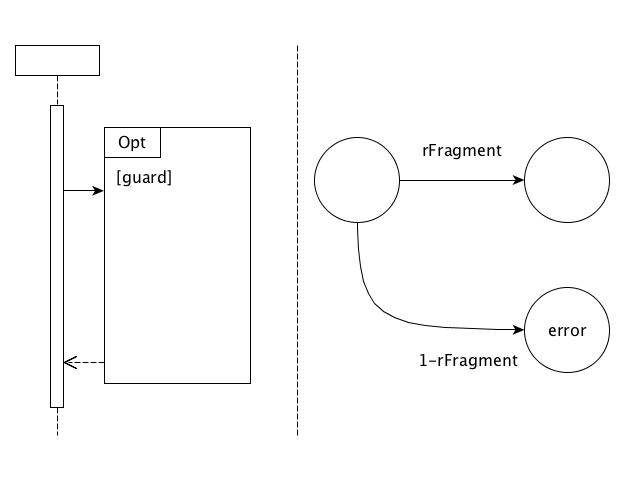
\includegraphics[width=0.7\columnwidth]{img/SD_opt_fragment}
%\caption{Transformation of optional combined fragment into FDTMC.}
%\label{fig:SD_opt_fragment}
%\end{figure}


\begin{figure}[!hbt]
  \centering
  \begin{subfigure}[t]{\textwidth}
    \resizebox{\linewidth}{!}{
	    \centering
	    \begin{tikzpicture}[x=1.5cm]
\centering
%%%%%%%%%%%%%%%%%%%%%%%% help lines
%\draw[help lines] (0,0) grid +(6,2);

%%%%%%%%%%%%%%%%%%%%%%%% nodes
\node[initial](initial) at (0,1) {(\textit{init})};
\node[](capt) at (1,1){};
\node[](situ) at (2,1){};
\node[](qosg) at (3,1){};
\node[](deci) at (4,1){};
\node[](reco) at (5,1){};
\node[](merg) at (6,1){};
\node[success](success) at (7.5,1){(\textit{success})};

%%%%%%%%%%%%%%%%%%%%%%%% edges
\draw[thick, -{latex[width=3mm]}] (initial) to node[draw=none, rotate=45, yshift=0.6cm, xshift=0.8cm]{\scriptsize $rCapture$}  (capt);
\draw[thick, -{latex[width=3mm]}] (capt) -- node[draw=none, rotate=45, yshift=0.6cm, xshift=0.8cm]{\scriptsize $rSituation$} (situ);
\draw[thick, -{latex[width=3mm]}] (situ) --  node[draw=none, rotate=45, yshift=0.6cm, xshift=0.8cm]{\scriptsize $rQosGoal$}(qosg);
\draw[thick, -{latex[width=3mm]}, line width=3pt] (qosg) --  node[draw=none, rotate=45, above, xshift=0.3cm]{\scriptsize $0.5$}(deci);
\draw[thick, -{latex[width=3mm]}] (deci) --  node[draw=none, rotate=45, yshift=0.4cm, xshift=1.2cm]{\scriptsize $rReconfiguration$}(reco);
\draw[thick, -{latex[width=3mm]}] (reco) --  node[draw=none, rotate=45, yshift=0.4cm, xshift=0.2cm]{\scriptsize $1.0$}(merg);
\draw[thick, -{latex[width=3mm]}] (merg) --  node[draw=none, rotate=45, yshift=0.4cm, xshift=0.2cm]{\scriptsize $1.0$}(success);

\draw[thick, line width=2pt, dashed, -{latex[width=3mm]}] (qosg) -- +(0,-1cm) -|  node[draw=none, rotate=45, above, near start]{\scriptsize $0.5$} (merg);
\path[-{latex[width=3mm]}] (success) edge [loop right] node [draw=none]{$1.0$}();
\end{tikzpicture}


    }
    \caption{FDTMC of the control loop of BSN-SPL.}
    \label{fig:bsnControlLoopFDTMC}
  \end{subfigure}

  \begin{subfigure}[t]{\textwidth}
    \resizebox{\linewidth}{!}{
	    \centering
	    \begin{tikzpicture}[x=1.5cm]
\centering
%%%%%%%%%%%%%%%%%%%%%%%% help lines
%\draw[help lines] (0,0) grid +(5,2);

%%%%%%%%%%%%%%%%%%%%%%%% nodes
\node[initial](initial) at (-0.5,1) {(\textit{init})};
\node[](s1) at (1,1){};
\node[](s2) at (2,1){};
\node[](s3) at (3,1){};
\node[](s4) at (4,1){};
\node[success](success) at (5.5,1){(\textit{success})};


%%%%%%%%%%%%%%%%%%%%%%%% edges
\draw[thick, -{latex[width=3mm]}] (initial) -- node[draw=none, rotate=45, yshift=0.6cm, xshift=0.8cm]{\scriptsize rOxygenation} (s1);
\draw[thick, -{latex[width=3mm]}] (s1) -- node[draw=none, rotate=45, yshift=0.6cm, xshift=0.8cm]{\scriptsize rPulseRate} (s2);
\draw[thick, -{latex[width=3mm]}] (s2) -- node[draw=none, rotate=45, yshift=0.6cm, xshift=0.8cm]{\scriptsize rTemperature} (s3);
\draw[thick, -{latex[width=3mm]}] (s3) -- node[draw=none, rotate=45, yshift=0.6cm, xshift=0.8cm]{\scriptsize rPosition} (s4);
\draw[thick, -{latex[width=3mm]}] (s4) -- node[draw=none, rotate=45, yshift=0.6cm, xshift=0.5cm]{\scriptsize rFall} (success);

\path[-{latex[width=3mm]}] (success) edge [loop right] node [draw=none]{$1.0$}();
\end{tikzpicture}


    }
    \caption{FDTMC of \underline{situation} sequence diagram.}
    \label{fig:situationFDTMC}
  \end{subfigure}

  \begin{subfigure}[t]{\textwidth}
    \resizebox{\linewidth}{!}{
	    \centering
	    \begin{tikzpicture}[x=1.3cm]
\centering
%%%%%%%%%%%%%%%%%%%%%%%% help lines
%\draw[help lines] (0,0) grid +(9,2);

%%%%%%%%%%%%%%%%%%%%%%%% nodes
\node[initial](initial) at (-0.5,1) {(\textit{init})};
\node[](s1) at (1,1){};
\node[](s2) at (2,1){};
\node[](s3) at (3,1){};
\node[](s4) at (4,1){};
\node[](s5) at (5,1){};
\node[](s6) at (6,1){};
\node[](s7) at (7,1){};
\node[](s8) at (8,1){};
\node[success](success) at (9.5,1){(\textit{success})};


%%%%%%%%%%%%%%%%%%%%%%%% edges
\draw[thick, -{latex[width=3mm]}] (initial) -- node[draw=none, rotate=45, yshift=0.6cm, xshift=0.5cm]{$0.999$} (s1);
\draw[thick, -{latex[width=3mm]}] (s1) -- node[draw=none, rotate=45, yshift=0.6cm, xshift=0.5cm]{$0.999$} (s2);
\draw[thick, -{latex[width=3mm]}] (s2) -- node[draw=none, rotate=45, yshift=0.6cm, xshift=0.5cm]{$0.999$} (s3);
\draw[thick, -{latex[width=3mm]}] (s3) -- node[draw=none, rotate=45, yshift=0.6cm, xshift=0.5cm]{$0.999$} (s4);
\draw[thick, -{latex[width=3mm]}] (s4) -- node[draw=none, rotate=45, yshift=0.6cm, xshift=0.5cm]{$rSqlite$} (s5);
\draw[thick, -{latex[width=3mm]}] (s5) -- node[draw=none, rotate=45, yshift=0.6cm, xshift=0.5cm]{$rMemory$} (s6);
\draw[thick, -{latex[width=3mm]}] (s6) -- node[draw=none, rotate=45, yshift=0.6cm, xshift=0.5cm]{$0.999$} (s7);
\draw[thick, -{latex[width=3mm]}] (s7) -- node[draw=none, rotate=45, yshift=0.6cm, xshift=0.5cm]{$0.999$} (s8);
\draw[thick, -{latex[width=3mm]}] (s8) -- node[draw=none, rotate=45, yshift=0.6cm, xshift=0.5cm]{$0.999$} (success);

\path[-{latex[width=3mm]}] (success) edge [loop above] node [draw=none]{$1.0$}();

\end{tikzpicture}


    }
    \caption{FDTMC of oxygenation sequence diagram.}
    \label{fig:oxygenationFDTMC}
  \end{subfigure}

  \begin{subfigure}[t]{0.5\textwidth}
    \resizebox{\linewidth}{!}{
	    \centering
	    \begin{tikzpicture}[x=1.5cm]
%%%%%%%%%%%%%%%%%%%%%%%% help lines
%\draw[help lines] (0,0) grid +(6,2);

%%%%%%%%%%%%%%%%%%%%%%%% nodes
\node[initial](initial) at (0,1) {(\textit{init})};
\node[](s1) at (1,1){};
\node[success](success) at (2.2,1){(\textit{success})};

%%%%%%%%%%%%%%%%%%%%%%%% edges
\draw[thick, -{latex[width=3mm]}] (initial) -- node[draw=none, rotate=45, yshift=0.3cm, xshift=0.8cm]{\scriptsize $0.999$}  (s1);
\draw[thick, -{latex[width=3mm]}] (s1) -- node[draw=none, rotate=45, yshift=0.3cm, xshift=0.8cm]{\scriptsize $0.999$} (success);
\path[-{latex[width=3mm]}] (success) edge [loop right] node [draw=none]{$1.0$}();
\end{tikzpicture}


    }
    \caption{FDTMC of SQLite/Memory sequence diagram.}
    \label{fig:persistenceFDTMC}
  \end{subfigure}
\centering
\caption{Resulting FDTMCs.}
\label{fig:resultingFDTMCs}
\end{figure}

As an example, Figure \ref{fig:rdgOxygenation} shows an excerpt of the RDG
corresponding to the UML activity and sequence diagrams depicted in
figures~\ref{fig:bsnControlLoop}, \ref{fig:oxygenationSituation} and
\ref{fig:temperatureSituation} such there is an RDG node for each kind of
behavioral fragment  found on all figures. Note that whenever a behavioral
fragment (activity or sequence diagrams and optional combined fragment) has to
be transformed, its RDG node and an edge are created to accommodate its FDTMC
and represent the behavioral dependency, respectively.  The node labeled
\texttt{rRoot} is the root node of this RDG.  The FDTMC assigned to this node
(Figure~\ref{fig:bsnControlLoopFDTMC}) is built by applying the transformation
rules presented by Section~\ref{subsec:transfomrationRulesActivityDiagramElements}  to the activity diagram in
Figure~\ref{fig:bsnControlLoop}.  The decision node in this activity diagram
gives rise to the bold and dashed transitions in
Figure~\ref{fig:bsnControlLoopFDTMC}, representing the \textit{yes} and
\textit{no} branches.


The RDG node \texttt{rSituation} represents the sequence diagrams depicted in
figures~\ref{fig:oxygenationSituation} and \ref{fig:temperatureSituation},
corresponding to the activity \emph{System identifies \underline{situation}} of
BSN's control loop (Figure~\ref{fig:bsnControlLoop}).  Since this activity is
performed by all products, its presence condition is \textit{true}.  The node's
FDTMC, depicted in Figure~\ref{fig:situationFDTMC}, is obtained from the
sequence diagram according to the transformation templates presented by Section~\ref{subsec:transformationRulesSequenceDiagramElements}.  The outgoing edges of the node
\texttt{rSituation} in Figure \ref{fig:rdgOxygenation} correspond to its
dependency on the availability of sensor information---one RDG node per
optional behavioral fragment.  (Most of such RDG nodes corresponding to such
behavioral fragments are omitted for brevity).

The node labeled \texttt{rOxygenation} in Figure \ref{fig:rdgOxygenation}
represents the behavior in the behavioral fragment whose presence condition is
\textit{oxygenation} (Figure \ref{fig:oxygenationSituation}).  The corresponding
FDTMC is presented in Figure~\ref{fig:oxygenationFDTMC}.
% The reliability computed for this FDTMC by the reachability definition,
% results into the following formula
%
% \footnotesize
% \begin{align}
% f'(oxygenation) & =  0.999 \cdot 0.999 \cdot 0.999 \cdot 0.999 \cdot rSqlite
% \cdot rMemory \cdot 0.999 \cdot 0.999 \cdot \nonumber \\
%                 & = 0.999^6 \cdot rSqlite \cdot rMemory \nonumber 
% \end{align}
% \normalsize
% that is defined in terms of the reliabilities computed for the optional combined
% fragments associated to the persistence ways.
The node \texttt{rOxygenation} depends on two basic RDG nodes, \texttt{rSqlite}
and \texttt{rMemory}, corresponding to the nested behavioral fragments whose
presence conditions are \textit{sqlite} and \textit{memory}, respectively.
Since both fragments have similar behavior (two sequential messages, each with
reliability $0.999$) their corresponding FDTMCs are equal
(Figure~\ref{fig:persistenceFDTMC}).


Finally, the approach relies on the divide-and-conquer strategy to decompose
behavioral models. During the transformation of a behavioral fragment into an
FDTMC, whenever another behavioral fragment is found, an RDG node is created
with a parent-child dependency relation with the parent's RDG node.  The way a
software product line is decomposed results into a tree-like RDG if there is no
behavioral fragment being reused. Otherwise, an  RDG node representing a reused
behavior fragment will have as many incoming edges as the times the fragment is
reused. In this specific case, the structure of the resulting RDG will not be
tree-like (that is why the RDG is a directed acyclic graph, in general). 

% Applying the reachability measure definition on such FDTMC, it results into
% the following expression 

% \scriptsize
% \begin{align}
% 	f'(rSqlite) = f'(rMemory)& = 0.999 \cdot 0.999 \nonumber \\
% 	                         & = 0.999^2 \nonumber
% \end{align}
% \normalsize

\begin{figure}[!hbt] 
  \centering 
  \begin{subfigure}[t]{0.50\columnwidth}
    \centering 
%    \includegraphics[scale=0.45, keepaspectratio=true]
%      {img/rdgBeforeFeatureBasedAnalysis}
    \resizebox{\linewidth}{!}{
	    \centering 
	    \begin{tikzpicture}[
	baseline,
	level distance=20mm,
        text depth=.1em, 
        text height=.8em,
	level 2/.style={sibling distance=5em},
        level 3/.style={sibling distance=10em}]
   \node[minimum size=2cm]{rRoot}
   child[->, thick]{node[minimum size=2cm]{rSituation}
         child{node[minimum size=2cm]{rOxygenation}
            child{node(rsqlite)[minimum size=2cm]{rSqlite}}
            child{node(rmemory)[minimum size=2cm]{rMemory}}}
         child{node[draw=none]{$\dots$}}
         child{node[draw=none]{$\dots$}}
	 child{node[draw=none]{$\dots$}}
     child{node(rtemperature)[]{$rTemperature$}}}
      child[->, thick]{node[draw=none]{$\dots$}} 
      child[->, thick]{node[draw=none]{$\dots$}} 
      child[->, thick]{node[draw=none]{$\dots$}};
   \draw[->,thick] (rtemperature) to [bend left=30](rmemory);
   \draw[->,thick] (rtemperature) to [bend left=45](rsqlite);
\end{tikzpicture}


    }    
    \caption{RDG nodes.} 
    \label{fig:rdgOxygenation}	
  \end{subfigure}
  \vspace{1cm}

  \begin{subfigure}[t]{0.80\columnwidth} 
    \resizebox{\linewidth}{!}{
	    \centering 
	    \begin{tikzpicture}[
	baseline,
	level distance=20mm,
        text depth=.1em, 
        text height=.10em,
	level 2/.style={sibling distance=7em},
        level 3/.style={sibling distance=10em}]
   \node[rectangle, minimum height=1.0cm, draw=none]{$\begin{aligned}
	   \varepsilon(\mathit{rRoot}) =& 0.5 \cdot \mathit{rCapture} \cdot \mathit{rSituation} \cdot \mathit{rQosGoal} \\
       +& 0.5 \cdot \mathit{rCapture} \cdot \mathit{rSituation} \cdot \mathit{rQosGoal} \cdot \mathit{rReconfiguration}
       \end{aligned}$}
   child[->,thick]{node[minimum width=2cm,rectangle, draw=none]{$\varepsilon(\mathit{rSituation})= \dots$}
            child{node[minimum width=2cm, minimum height= 1.3cm, rectangle, draw=none]{$\begin{aligned}
       \varepsilon(\mathit{rOxygenation})= & \\ 0.999^7 \cdot  
                                          \mathit{rSqlite} \cdot \mathit{rMemory}
            \end{aligned}$}
            child{node(rsqlite)[minimum width=2cm,rectangle, draw=none]{$\varepsilon(\mathit{rSqlite})=0.999^2$}}
            child{node(rmemory)[minimum width=2cm,rectangle, draw=none]{$\varepsilon(\mathit{rMemory})=0.999^2$}}}
         child{node[minimum width=2cm,rectangle, draw=none]{$\dots$}}
         child{node[minimum width=2cm,rectangle, draw=none]{$\dots$}}
	 child{node[minimum width=2cm,rectangle, draw=none]{$\dots$}}
	 child{node(rtemperature)[minimum width=2cm, minimum height=1.3cm, rectangle, draw=none]{$\begin{aligned}& \varepsilon(\mathit{rTemperature})= \\
      	                                                         & 0.999^7 \cdot \mathit{rSqlite} \cdot \mathit{rMemory} \end{aligned}$}}}
      child[->, thick]{node[minimum width=2cm,rectangle, draw=none]{$\dots$}} 
      child[->, thick]{node[minimum width=2cm,rectangle, draw=none]{$\dots$}} 
      child[->, thick]{node[minimum width=2cm,rectangle, draw=none]{$\dots$}};
      
      \draw[->,thick] (rtemperature.south) to [bend left=30](rmemory);
   \draw[->,thick] (rtemperature.south) to [bend left=45](rsqlite.south);
\end{tikzpicture}

    }    
    \caption{Dependencies between expressions.} 
    \label{fig:formulaeDependencies}
  \end{subfigure}
  \vspace{0.3cm} \caption{RDG excerpt for the BSN product line.}
  \label{fig:bsnRdg}
\end{figure}







%%%%%%%%%%%%%%%%%%%%%%%%%%%%%%%%%%%%%%%%%%%%%%%%%%%%%%%%%%%%%%%%%%%%%%%%%%%%%%%%
%% FEATURE-BASED ANALYSIS
%%%%%%%%%%%%%%%%%%%%%%%%%%%%%%%%%%%%%%%%%%%%%%%%%%%%%%%%%%%%%%%%%%%%%%%%%%%%%%%%
\section{Feature-Based analysis \label{sec:featureBasedAnalysis}}


The role of the feature-based analysis step is to analyze the FDTMC for each RDG
node in isolation, abstracting from the dependencies to other RDG nodes.  That
is, instead of evaluating a potentially intractable FDTMC for the product line
as a whole, the approach performs multiple evaluations of smaller models, one
per behavioral fragment.
%The evaluation consists on evaluate the probabilistic property model just by
%considering its interfaces. As all $I_{fragment}$ interfaces have a state
%representing its successful execution, the same PCTL property can be used for
%all FDTMCs, which is given by the property of eventually reaching the success
%final state ($P=(\diamondsuit success)$).  The result for feature-based
%evaluation dimension is a parametric formula describing its reliability where
%parameters represents the reliabilities of RDG nodes it depends on. 

For each RDG node $x \in \mathcal{N}$, its FDTMC is subject to  parametric model
checking~\cite{Hahn_param_2010,Filieri_pmctool_2012}. This feature-based
analysis yields $x$'s reliability as an expression over the reliabilities of the
$n$ RDG nodes $x_1, \dotsc, x_n$, on which it depends.  This expression is
denoted by a function $[0,1]^n \to [0,1]$, that is, the computation of a
reliability value takes $n$ reliability values as input. Therefore, there is a
function $\varepsilon: \mathcal{N} \to ([0,1]^n \to [0,1])$ that yields the
semantics of the reliability expression for a given RDG node.  To remove
possible ambiguities, the order of the formal parameters is determined by a
total order relation over the corresponding RDG nodes $x_i$.  When analyzing RDG
nodes, the same reliability property of eventually reaching the \emph{success}
final state (expressed by the model checker query expression
$P_{=?}[\diamondsuit \mathit{``success"}]$---see
Section~\ref{subsec:softwareReliability}) is used for all FDTMCs.

Performing feature-based analysis over the RDG, as depicted in
Figure~\ref{fig:rdgOxygenation}, yields the expressions shown in
Figure~\ref{fig:formulaeDependencies}.
%\begin{align*} f'(Oxygenation) &= 995*Sqlite*Memory/1000 \\ f'(Sqlite) &=
%998/1000\\f'(Memory) &= 998/1000 \end{align*}
These expressions illustrate that basic nodes have their reliabilities defined
in terms of constants, whereas the reliabilities of variant nodes ultimately
depend on the ones of basic RDG nodes.  For the sake of simplicity, we overload
the names of RDG nodes in Figure~\ref{fig:rdgOxygenation} as variables in the
expressions in Figure~\ref{fig:formulaeDependencies}.  This way, we map each
variable to the RDG node whose reliability it represents.
%For the sake of simplicity, we are overloading the names of RDG nodes in
%Figure~\ref{fig:rdgOxygenation} and the expressions' variables in
%Figure~\ref{fig:formulaeDependencies}. From now on, whenever a name regarding
%the Figure~\ref{fig:rdgOxygenation} is mentioned it represents an RDG node,
%whereas a name regarding the Figure~\ref{fig:formulaeDependencies} represents
%an expression variable. Therefore, the rationale for such names overloading is
%that each expression's variable in Figure~\ref{fig:formulaeDependencies}
%represents the reliability values of its corresponding node in
%Figure~\ref{fig:rdgOxygenation}. 

%Although there is no need to define an order to evaluate the RDG nodes, as the
%feature-based dimension abstracts the dependencies among behavior fragments,
%the RDG nodes are evaluated following a total order defined by the RDG
%topology. For each behavior dependency found at behavioral models, there is a
%parameter representing the reliability its respective behavior fragment may
%assume, and there is an edge from the RDG node to the RDG node containing the
%behavior fragment it depends on. 








%%%%%%%%%%%%%%%%%%%%%%%%%%%%%%%%%%%%%%%%%%%%%%%%%%%%%%%%%%%%%%%%%%%%%%%%%%%%%%%%
%% FAMILY-BASED ANALYSIS
%%%%%%%%%%%%%%%%%%%%%%%%%%%%%%%%%%%%%%%%%%%%%%%%%%%%%%%%%%%%%%%%%%%%%%%%%%%%%%%%
\section{Family-Based Analysis \label{sec:familyBasedAnalysis}}

The possible next step would be to evaluate the obtained expressions once for
each valid configuration, so that the reliability of every product would be
computed.  This enumerative approach would be, in fact, a \emph{product-based}
analysis, yielding an overall \emph{feature-product-based} analysis, similar to
the one described by \citet{ghezzi_model-based_2013}.  However, evaluating all
products using this approach would be still prone to an exponential blowup,
which would harm scalability.

To avoid this problem, the method hereby presented leverages a family-based
analysis strategy to \emph{lift} each expression to perform arithmetic
operations over variational data, with the help of an appropriate
\emph{variational data structure}~\cite{walkingshaw_variational_2014}.  This
way, it is able to represent all possible values under variation and efficiently
evaluate results, sharing computations whenever possible.  The data structure of
choice is the Algebraic Decision Diagram (ADD)\footnotemark{}~\cite{Iris1993},
because it efficiently encodes a Boolean function $\mathbb{B}^n \to \mathbb{R}$.
This is the same type as a mapping from configurations to reliability values
would have, provided the Boolean values $b_1, \dotsc, b_n \in
{\mathbb{B}=\{0,1\}}$ are taken to denote the presence (or absence) of the
corresponding features $f_1, \dotsc, f_n \in F$ (where $F$ is the set of
features in the feature model).
\footnotetext{% ADDs, also called Multi-Terminal Binary Decision Diagrams
	(MTBDD), generalize Binary Decision Diagrams (BDD) to Real-valued
	Boolean functions.
%
}

Given an expression $\varepsilon(x)$, obtained for an RDG node $x$ in the
feature-based step of the analysis (Section \ref{sec:featureBasedAnalysis}),
the reliability ADD $\alpha(x)$ is obtained by first valuating the parameters
$x_1, \dotsc, x_k$ of the lifted expression with the ADDs for the reliabilities
$\alpha(x_1), \dotsc, \alpha(x_k)$ of the corresponding nodes upon which $x$
depends.  Then, arithmetic operations are performed using ADD semantics: for
ADDs $A_1$ and $A_2$ over $k$ Boolean variables and a binary operation $\odot
\in \{+, -, \cdot, \div\}$, $(A_1 \odot A_2)(b_1,\dotsc,b_k) =
A_1(b_1,\dotsc,b_k) \odot A_2(b_1,\dotsc,b_k)$.

However, the computation of $\alpha(x)$ must take presence conditions into
account.  To accomplish this, the method constrains the valuation of a variable
$x_i$ with an ADD $p_{x}: \llbracket \mathit{FM} \rrbracket \to \mathbb{B}$
encoding its presence condition, with $x$ ranging over $x_1$ to $x_n$, such $n$
is the number of features.  This ADD has the property that all configurations $c
\in \llbracket \mathit{FM} \rrbracket$ that satisfy $x_i$'s presence condition
evaluate to $1$, while all others evaluate to $0$.  The resulting constrained
decision diagram $\varphi_{x_i}$ is given by:

\begin{align*}
  \varphi_{x_i}(c) = \begin{cases}
    \alpha(x_i)(c) &\mbox{if} \, p_{x_i}(c) = 1 \\
    1 &\mbox{otherwise}
  \end{cases}
\end{align*}

Notice the attribution of  $1$ to the reliability of a behavior that is absent
in a given configuration.  The intuition is that, for those configurations that
do not satisfy the fragment's guard conditions (i.e., $p_{x_i}(c) = 0$), the
behavior represented by the optional fragment will not be part of the resulting
product's behavior.  Since an absent behavioral fragment has no influence on the
reliability of the overall system, in practice it can be assumed $1.0$ as its
reliability value (i.e., it cannot fail).  The ADD $\varphi_{x_i}$ is obtained
by means of the \emph{if-then-else} operator for decision diagrams, and the
operational details of this construction are presented in
Section~\ref{subsec:reana}.

This method of evaluating the expressions is inherently recursive, since the
resulting value of computing the expression for a given RDG node depends on the
results of computing the expressions for the nodes on which it depends.  For
example, Figure \ref{fig:formulaeDependencies} shows that the expression
$\varepsilon(\mathtt{rOxygenation})$ is defined in terms of the variables
\texttt{rSqlite} and \texttt{rMemory}.  Thus, before computing the lifted
counterpart of expression $\varepsilon(\mathtt{rOxygenation})$, it is necessary
to compute the lifted counterparts of expressions
$\varepsilon(\mathtt{rSqlite})$ and $\varepsilon(\mathtt{rMemory})$. The same
rationale holds for the \texttt{rTemperature} node, however the
$\alpha(\mathtt{rSqlite})$ and $\alpha(\mathtt{rMemory})$ are already computed and
thus they can be reused. In a brief,
the family-based step computes the reliabilities values each RDG node may assume
by solving its $\varepsilon$ expression using reliabilities values encoded by
$\alpha$ for the nodes it depends on. Thus, it follows that the reliability of
the product line as a whole is given by the ADD resulting from the computation
of $\alpha({\mathtt{rRoot}})$, where \texttt{rRoot} is the root RDG node.

\begin{figure}[p]
\centering
\begin{subfigure}[t]{0.7\columnwidth}
\resizebox{\linewidth}{!}{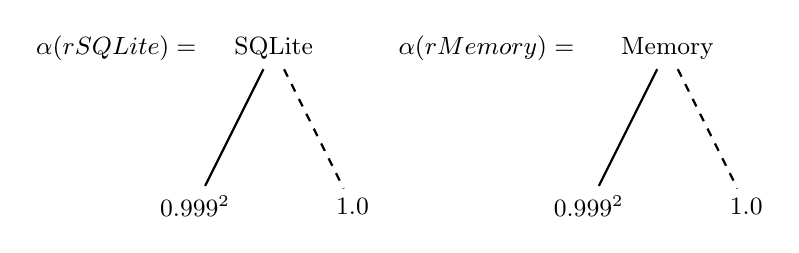
\begin{tikzpicture}[thick]
\centering
\small
\node[draw=none](alphaSqlite) at (-1,2) {$\alpha(rSQLite)=$};
\node(sqlite) at (1,2) {SQLite};
\node[rectangle, draw=none](rSqlite) at (0,0) {$0.999^2$};
\node[rectangle, draw=none](!rSqlite) at (2,0) {$1.0$};
\draw[thick] (sqlite) -- (rSqlite);
\draw[thick, dashed] (sqlite) -- (!rSqlite);

\node(memory) at (6,2) {Memory};
\node[draw=none](alphaMemory) at (3.7,2) {$\alpha(rMemory)=$};
\node[rectangle, draw=none](rMemory) at (5,0) {$0.999^2$};
\node[rectangle, draw=none](!rMemory) at (7,0) {$1.0$};
\draw[thick] (memory) -- (rMemory);
\draw[thick, dashed] (memory) -- (!rMemory);
\end{tikzpicture}
}
\caption{ADDs for $rSQlite$ and $rMemory$ nodes, respectively.}
\label{fig:addSqliteMemory}
\end{subfigure}
\vspace{0.5cm}

\begin{subfigure}[b]{0.40\textwidth}
\resizebox{\columnwidth}{!}{\begin{tikzpicture}[thick]
\small
\centering
\node[rectangle, draw=none] at (0,6.5) {$\alpha(rOxygenation)=$};
\node(oxygenation) at (3,6.5) {Oxygenation};
\node(sqlite) at (3,4) {SQLite};
\node(memory1) at (2,2) {Memory};
\node(memory2) at (4,2) {Memory};
\node[rectangle, draw=none](rOxygenation) at (2,0) {$0.999^5 \times 0.999^2$ \\ $=0.999^7$};
\node[rectangle, draw=none](invConfig) at (4,0) {$0.0$};
\node[rectangle, draw=none](absFrag) at (6,0) {$1.0$};

\draw(oxygenation) -- (sqlite);
\draw[dashed, bend left](oxygenation) to (absFrag.north);
\draw[dashed](sqlite) -- (memory1);
\draw(sqlite) -- (memory2);
\draw(memory1) -- (rOxygenation);
\draw[dashed](memory1) -- (invConfig);
\draw[dashed](memory2) -- (rOxygenation);
\draw(memory2) -- (invConfig);
\end{tikzpicture}
}
\caption{ADDs for $rOxygenation$ node.}
\label{fig:addOxygenation}
\end{subfigure}
~
\begin{subfigure}[b]{0.40\textwidth}
\resizebox{\columnwidth}{!}{\begin{tikzpicture}[thick]
\small
\centering
\node[rectangle, draw=none] at (0,6.5) {$\alpha(rTemperature)=$};
\node(temperature) at (3,6.5) {Temperature};
\node(sqlite) at (3,4) {SQLite};
\node(memory1) at (2,2) {Memory};
\node(memory2) at (4,2) {Memory};
\node[rectangle, draw=none](rTemperature) at (2,0) {$0.999^5 \times 0.999^2$ \\ $=0.999^7$};
\node[rectangle, draw=none](invConfig) at (4,0) {$0.0$};
\node[rectangle, draw=none](absFrag) at (6,0) {$1.0$};

\draw(temperature) -- (sqlite);
\draw[dashed, bend left](temperature) to (absFrag.north);
\draw[dashed](sqlite) -- (memory1);
\draw(sqlite) -- (memory2);
\draw(memory1) -- (rTemperature);
\draw[dashed](memory1) -- (invConfig);
\draw[dashed](memory2) -- (rTemperature);
\draw(memory2) -- (invConfig);
\end{tikzpicture}
}
\caption{ADDs for $rTemperature$ node.}
\label{fig:addTemperature}
\end{subfigure}
\vspace{0.5cm}


\begin{subfigure}[b]{\textwidth}
\centering
\resizebox{9cm}{!}{\footnotesize
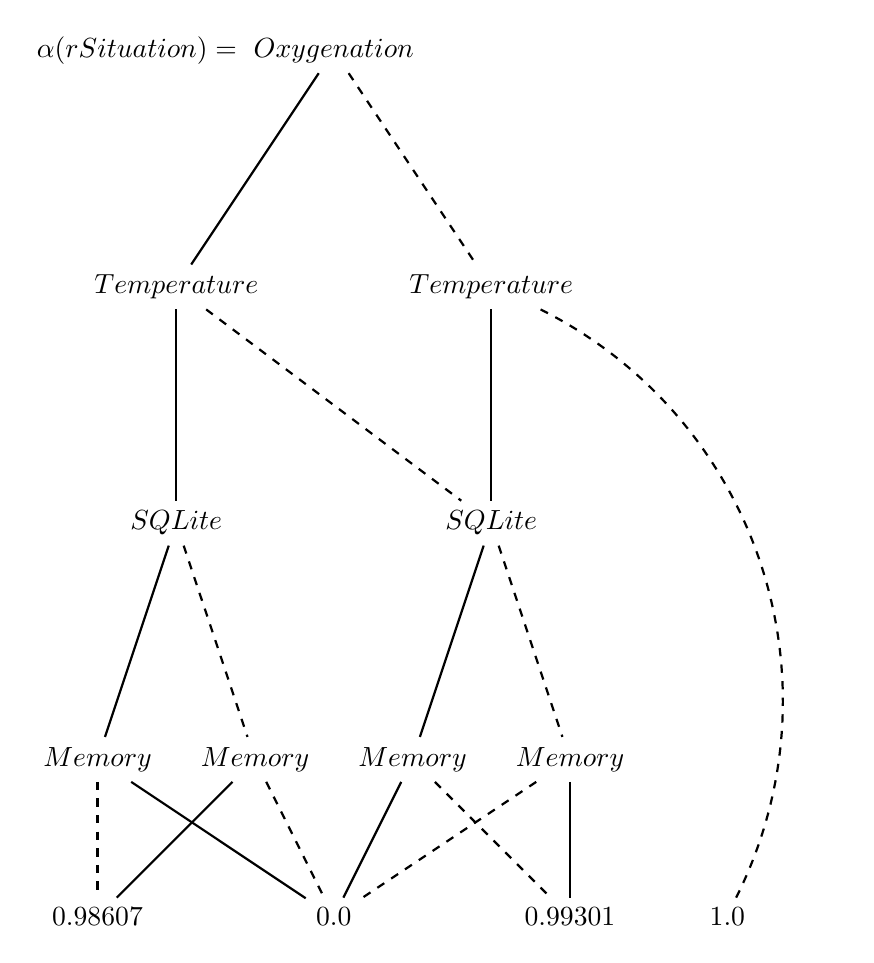
\begin{tikzpicture}[thick]
%\draw[help lines, step=1cm] (0,0) grid +(14,12);
\node[rectangle,draw=none](alpha) at (1.5,12) {$\alpha(rSituation)=$};
\node(o1) at (4,12) {$Oxygenation$};
\node(t1) at (2,9) {$Temperature$};
\node(t2) at (6,9) {$Temperature$};
\node(sq1) at (2,6) {$SQLite$};
\node(sq2) at (6,6) {$SQLite$};
\node(m1) at (1,3) {$Memory$};
\node(m2) at (3,3) {$Memory$};
\node(m3) at (5,3) {$Memory$};
\node(m4) at (7,3) {$Memory$};
\node[rectangle, draw=none](tr1) at (1,1) {$0.98607$};
\node[rectangle, draw=none](tr2) at (4,1) {$0.0$};
\node[rectangle, draw=none](tr3) at (7,1) {$0.99301$};
\node[rectangle, draw=none](tr4) at (9,1) {$1.0$};

\draw(o1)--(t1);
\draw[dashed](o1)--(t2);
\draw(t1)--(sq1);
\draw[dashed](t1)--(sq2);
\draw(t2)--(sq2);
\draw[dashed](t2) to [bend left=45](tr4);
\draw(sq1)--(m1);
\draw[dashed](sq1)--(m2);
\draw(sq2)--(m3);
\draw[dashed](sq2)--(m4);
\draw[dashed](m1)--(tr1);
\draw(m1)--(tr2);
\draw(m2)--(tr1);
\draw[dashed](m2)--(tr2);
\draw(m3)--(tr2);
\draw[dashed](m3)--(tr3);
\draw[dashed](m4)--(tr2);
\draw(m4)--(tr3);
\end{tikzpicture}
\normalsize
}
\caption{ADDs for $rSituation$ node.}
\label{fig:addSituation}
\end{subfigure}

\caption{ADDs for the running example.}
\label{fig:addRunningExample}
\end{figure}

Naturally, basic nodes are the base case of this recursion, since, by
definition, they depend on no other node. Figure~\ref{fig:addSqliteMemory}
depicts the ADDs representing the reliability enconding of the RDG nodes
\texttt{rSqlite} and \texttt{rMemory}, respectively. Each ADD node represents a
feature whose continuous edge denotes the feature's presence at the
configuration, meanwhile the dashed edge means the feature is absent.
Thus, $\alpha(\mathtt{rSqlite})$ encodes the RDG node assumes the reliability
value $0.999^2$ when the feature \emph{Sqlite} is part of the configuration,
otherwise $1.0$. In an analogous way, the ADD for the \texttt{rMemory} RDG node
represent its reliabilities values. 

Figure~\ref{fig:addOxygenation} shows the reliability encoding computed for the
\texttt{rOxygenation} RDG node. Since $\varepsilon(rOxygenation)$ is defined in
terms of the  variables representing the reliabilities of the nodes which it
depends, $\alpha(rOxygenation)$ is computed by assigning the ADDs previously
computed to \texttt{rSqlite} and \texttt{rMemory} to its respective variables in
$\varepsilon(\texttt{rOxygenation})$, which is solved by employing the ADD's
arithmetic. The resulting ADD is constrained to represent only the reliabilities
of valid configurations when it is multiplied by the ADD representing the
feature model's rules. In fact, all paths leading to non-zero terminal
represents a valid configuration. In the case the feature \emph{Oxygenation} is
absent, its influence on the configuration's reliability is null, thus
$\alpha(rOxygenation)$ assumes $1.0$.  Otherwise, for configurations containing
\emph{Oxygenation} and only one persistence feature (\emph{SQLite} or
\emph{Memory}), its respective path in the ADD leads to the reliability value
$0.999^7$. Finally, the paths leading to the reliability value $0$ represent an
ill-formed configuration. For example, since \emph{SQLite} and \emph{Memory} are
alternative features, the paths representing that both features are present or
absent will lead to $0$. The same rationale holds for the \texttt{rTemperature}
node whose ADD is represented by Figure~\ref{fig:addTemperature}. All these
cases are also represented by the Table~\ref{table:oxygenation-reliability}.
Note that when the feature \emph{Oxygenation} is absent for
$\alpha(\mathtt{rOxygenation})$ (or the feature \emph{Temperature} is absent
for $\alpha(\mathtt{rTemperature})$), the presence or absence of \emph{SQLite}
and \emph{Memory} are not considered. Such effect is expected because,
intuitively, since the fragment they are comprised is not part of the
configuration, the presence of such features have no effect at the reliability
computation.




%Table~\ref{table:oxygenation-reliability} presents some of the possible
%reliabilities of the node \texttt{rOxygenation}, that is,
%$\alpha(\mathtt{rOxygenation})(c)$ for chosen configurations $c \in \llbracket
%\mathit{FM} \rrbracket$.  For brevity, we represent configurations using the
%features of interest only. Given that this node depends on nodes for which the
%presence conditions are the atomic propositions \emph{sqlite} and
%\emph{memory}, which are alternative features, the computation of reliability
%for configurations in which these are not simultaneously selected is carried
%out as mentioned before.
%
%However, for configurations that do not respect this rule, the reliability is
%unspecified (represented by ``--'' in the table).  Even though individual
%presence conditions are satisfied in isolation, global consistency may still
%not be achieved.  This is why we must consider the variability model for the
%purpose of discarding invalid configurations. \textit{Configuration pruning} is
%the name of this family-based evaluation step where we discard the reliability
%values of ill-formed products by attributing the value \emph{0} to them at the
%resulting reliability ADD. In the previous example, the feature model presented
%in Figure~\ref{fig:fm} is violated for a configuration containing \emph{Sqlite}
%and \emph{Memory}, so this configuration is discarded (as shown by the last
%line of Table~\ref{table:oxygenation-reliability}).

\vspace{0.3cm}



\begin{table}[t]
\centering
\caption{Reliability of \texttt{rOxygenation}, \texttt{rTemperature} and \texttt{rSituation} fragments.}
\resizebox{\columnwidth}{!}{
\begin{tabular}{cc}
  \toprule
  Configuration ($c$)                     & $\alpha(\mathtt{rOxygenation})(c)$\\ 
  \midrule
  \{Oxygenation, Sqlite, $\lnot$Memory\}  & 995*(998/1000)*1/1000 = 0,99301   \\ 
  \{Oxygenation, $\lnot$Sqlite, Memory\}  & 995*1*(998/1000)/1000 = 0,99301   \\ 
  \{$\lnot$Oxygenation, \_\_\_, \_\_\_\}  & 1,0                               \\ 
  \{Oxygenation, Sqlite, Memory\}         & --                                \\ 
  \{Oxygenation, $\lnot$Sqlite, $\lnot$Memory\}         & --                                \\ 
  \midrule
  Configuration ($c$)                     & $\alpha(\mathtt{rTemperature})(c)$\\ 
  \midrule
  \{Temperature, Sqlite, $\lnot$Memory\}  & 995*(998/1000)*1/1000 = 0,99301   \\ 
  \{Temperature, $\lnot$Sqlite, Memory\}  & 995*1*(998/1000)/1000 = 0,99301   \\ 
  \{$\lnot$Temperature, \_\_\_, \_\_\_\}  & 1,0                               \\ 
  \{Temperature, Sqlite, Memory\}         & --                                \\ 
  \{Temperature, $\lnot$Sqlite, $\lnot$Memory\}         & --                                \\ 
  \midrule
  Configuration ($c$)                     & $\alpha(\mathtt{rSituation})(c)$\\ 
  \midrule
  \{Oxygenation, $\lnot$Temperature, Sqlite, $\lnot$Memory\}  & (99301/10000)*1 = 0,99301   \\ 
  \{Oxygenation, $\lnot$Temperature, $\lnot$Sqlite, Memory\}  & (99301/10000)*1 = 0,99301   \\ 
  \{Oxygenation, $\lnot$Temperature, Sqlite, Memory\}         & --                                \\ 
  \{Oxygenation, $\lnot$Temperature, $\lnot$Sqlite, $\lnot$Memory\}         & --                                \\ 
  \{$\lnot$Oxygenation, Temperature, Sqlite, $\lnot$Memory\}  & 1*(99301/10000) = 0,99301   \\ 
  \{$\lnot$Oxygenation, Temperature, $\lnot$Sqlite, Memory\}  & 1*(99301/10000) = 0,99301   \\ 
  \{$\lnot$Oxygenation, Temperature, Sqlite, Memory\}         & --                                \\ 
  \{$\lnot$Oxygenation, Temperature, $\lnot$Sqlite, $\lnot$Memory\}         & --                                \\ 
  \{Oxygenation, Temperature, Sqlite, $\lnot$Memory\}  & (99301/10000)*(99301/10000) = 0,98607   \\ 
  \{Oxygenation, Temperature, $\lnot$Sqlite, Memory\}  & (99301/10000)*(99301/10000) = 0,98607   \\ 
  \{Oxygenation, Temperature, Sqlite, Memory\}         & --                                \\ 
  \{Oxygenation, Temperature, $\lnot$Sqlite, $\lnot$Memory\}         & --                                \\ 
  \{$\lnot$Oxygenation, $\lnot$Temperature, \_\_\_, \_\_\_\}  & 1,0*1,0 = 1,0   \\ 
  \{$\lnot$Oxygenation, $\lnot$Temperature, \_\_\_, \_\_\_\}  & 1,0*1,0 = 1,0   \\ 
  \bottomrule
  \end{tabular}
}
\label{table:oxygenation-reliability}
\end{table}

Finally, in the case of the \texttt{rSituation} node, the
$\varepsilon(\mathtt{rSituation})$ is a formula expressed in terms of its
dependent nodes which \texttt{rOxygenation} and \texttt{rTemperature} comprise.
Thus, to solve $\alpha(rSituation)$ it is necessary assign the ADDs computed
for \texttt{rOxygenation} and \texttt{rTemperature} to its respective
variables. The resulting ADD is obtained by employing the ADD's arithmetic and
it is represented by the Figure~\ref{fig:addSituation}. Such diagram is also
constrained by the rules of the feature model expressed in its own ADD. Thus,
all paths leading to non-zero terminals are valid partial configurations,
otherwise, paths leading to the zero terminal represent ill-formed products.
All these possible cases are also represented by the
Table~\ref{table:oxygenation-reliability}.







%%%%%%%%%%%%%%%%%%%%%%%%%%%%%%%%%%%%%%%%%%%%%%%%%%%%%%%%%%%%%%%%%%%%%%%%%%%%%%%%
%% TOOL SUPPORT
%%%%%%%%%%%%%%%%%%%%%%%%%%%%%%%%%%%%%%%%%%%%%%%%%%%%%%%%%%%%%%%%%%%%%%%%%%%%%%%%
%\section{Tool support \label{sec:toolSupport}}










%%%%%%%%%%%%%%%%%%%%%%%%%%%%%%%%%%%%%%%%%%%%%%%%%%%%%%%%%%%%%%%%%%%%%%%%%%%%%%%%
%% CONCLUSION
%%%%%%%%%%%%%%%%%%%%%%%%%%%%%%%%%%%%%%%%%%%%%%%%%%%%%%%%%%%%%%%%%%%%%%%%%%%%%%%%
\section{Conclusion \label{sec:featureFamilyBasedConclusion}}

This chapter presented the evaluation method proposed for the reliability analysis of software product lines. Such method is comprised of three steps that initially, as shown by Listings\ref{lst:transformAD} and \ref{lst:transformSD}, is responsible for creating a runtime dependency graph from the behavioral models. Such step (ie. the transformation step) creates a node in the RDG for each behavioral fragment it founds while parsing the UML behavioral models. 

Meanwhile the transformation step, each RDG node receives its FDTMC created
according to the transformation rules afore presented. Such transformations
considers the behavioral elements in the scope of the behavioral fragment in
such a manner the resulting FDTMC is comprised of constants and variables that
abstract the nodes which it depends on. Then, the feature-based step employs
the parametrical model checker's algorithm in order to obtain the formula $\varepsilon$
representing the reliability of each node. Thus, this jointly use of
transformation and feature-based steps walk through the behavioral modeling in
a top-down fashion, in order to discover and transform the behavioral fragments
as soon as their dependencies are revealed.

When the RDG structure is finished, the family-based step takes place and runs
back all the runtime dependency graph in order to solve the reliability
expressions $\varepsilon$ taking into account the presence conditions
associated to each RDG node and the feature model's rules. The result is
represented in the suitable variational data structure named ADD such that, for
each RDG node, all valid partial configurations and their reliabilities are
represented by means of the $\alpha$ function (such function is represented by
the ADD). Thus, the family-based step follows a bottom-up strategy to solve all the expressions stored in RDG nodes, in such a manner that the $\alpha(root)$ stores the reliabilities of all full and valid configurations of the software product line.









